\section{Model2DRigid\-Lander  Class Reference}
\label{classModel2DRigidLander}\index{Model2DRigidLander@{Model2DRigid\-Lander}}
A rigid body with two small side thrusters, and a larger lower thruster. The goal is to navigate and softly \char`\"{}land\char`\"{} the craft by firing thrusters, in spite of gravity. 


{\tt \#include $<$model2d.h$>$}

Inheritance diagram for Model2DRigid\-Lander::\begin{figure}[H]
\begin{center}
\leavevmode
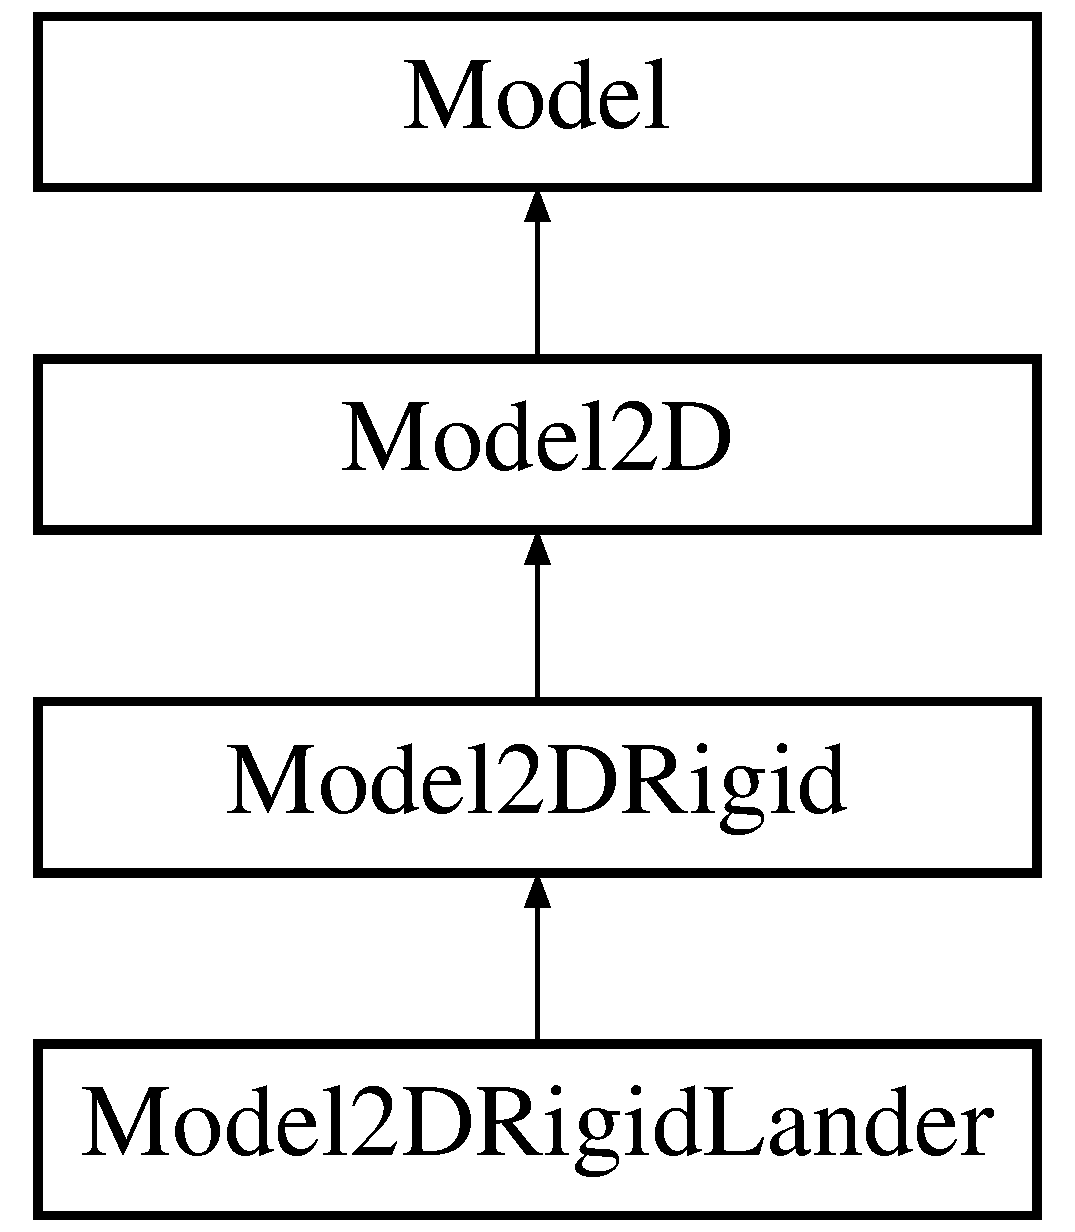
\includegraphics[height=4cm]{classModel2DRigidLander}
\end{center}
\end{figure}
\subsection*{Public Methods}
\begin{CompactItemize}
\item 
{\bf Model2DRigid\-Lander} (string path)
\item 
virtual {\bf $\sim$Model2DRigid\-Lander} ()
\item 
virtual {\bf MSLVector} {\bf State\-To\-Configuration} (const {\bf MSLVector} \&{\bf x})
\begin{CompactList}\small\item\em A method that converts a {\bf Model} {\rm (p.\,\pageref{classModel})} state in to a {\bf Geom} {\rm (p.\,\pageref{classGeom})} configuration.\item\end{CompactList}\item 
virtual {\bf MSLVector} {\bf State\-Transition\-Equation} (const {\bf MSLVector} \&{\bf x}, const {\bf MSLVector} \&u)
\begin{CompactList}\small\item\em The state transition equation, or equations of motion, xdot=f(x,u).\item\end{CompactList}\item 
virtual {\bf MSLVector} {\bf Integrate} (const {\bf MSLVector} \&{\bf x}, const {\bf MSLVector} \&u, const double \&h)
\begin{CompactList}\small\item\em Perform integration from state x, using input u, over time step h.\item\end{CompactList}\item 
{\bf MSLVector} {\bf Linear\-Interpolate} (const {\bf MSLVector} \&x1, const {\bf MSLVector} \&x2, const double \&a)
\begin{CompactList}\small\item\em Linearly interpolate two state while respecting topology.\item\end{CompactList}\item 
virtual {\bf MSLVector} {\bf State\-Difference} (const {\bf MSLVector} \&x1, const {\bf MSLVector} \&x2)
\begin{CompactList}\small\item\em Compute a {\bf MSLVector} {\rm (p.\,\pageref{classMSLVector})} based on x2-x1. In R$^\wedge$n, the states are simply subtracted to make the {\bf MSLVector} {\rm (p.\,\pageref{classMSLVector})}. This method exists to make things work correctly for other state-space topologies.\item\end{CompactList}\item 
virtual double {\bf Metric} (const {\bf MSLVector} \&x1, const {\bf MSLVector} \&x2)
\begin{CompactList}\small\item\em A distance metric, which is Euclidean in the base class.\item\end{CompactList}\end{CompactItemize}
\subsection*{Public Attributes}
\begin{CompactItemize}
\item 
double {\bf Mass}
\begin{CompactList}\small\item\em Mass in kg.\item\end{CompactList}\item 
double {\bf G}
\begin{CompactList}\small\item\em Accel of gravity (m/s$^\wedge$2).\item\end{CompactList}\item 
double {\bf Fs}
\begin{CompactList}\small\item\em Side thruster force.\item\end{CompactList}\item 
double {\bf Fu}
\begin{CompactList}\small\item\em Upward thruster force.\item\end{CompactList}\end{CompactItemize}


\subsection{Detailed Description}
A rigid body with two small side thrusters, and a larger lower thruster. The goal is to navigate and softly \char`\"{}land\char`\"{} the craft by firing thrusters, in spite of gravity.



\subsection{Constructor \& Destructor Documentation}
\index{Model2DRigidLander@{Model2DRigid\-Lander}!Model2DRigidLander@{Model2DRigidLander}}
\index{Model2DRigidLander@{Model2DRigidLander}!Model2DRigidLander@{Model2DRigid\-Lander}}
\subsubsection{\setlength{\rightskip}{0pt plus 5cm}Model2DRigid\-Lander::Model2DRigid\-Lander (string {\em path})}\label{classModel2DRigidLander_a0}


\index{Model2DRigidLander@{Model2DRigid\-Lander}!~Model2DRigidLander@{$\sim$Model2DRigidLander}}
\index{~Model2DRigidLander@{$\sim$Model2DRigidLander}!Model2DRigidLander@{Model2DRigid\-Lander}}
\subsubsection{\setlength{\rightskip}{0pt plus 5cm}virtual Model2DRigid\-Lander::$\sim$Model2DRigid\-Lander ()\hspace{0.3cm}{\tt  [inline, virtual]}}\label{classModel2DRigidLander_a1}




\subsection{Member Function Documentation}
\index{Model2DRigidLander@{Model2DRigid\-Lander}!Integrate@{Integrate}}
\index{Integrate@{Integrate}!Model2DRigidLander@{Model2DRigid\-Lander}}
\subsubsection{\setlength{\rightskip}{0pt plus 5cm}{\bf MSLVector} Model2DRigid\-Lander::Integrate (const {\bf MSLVector} \& {\em x}, const {\bf MSLVector} \& {\em u}, const double \& {\em h})\hspace{0.3cm}{\tt  [virtual]}}\label{classModel2DRigidLander_a4}


Perform integration from state x, using input u, over time step h.



Reimplemented from {\bf Model2DRigid} {\rm (p.\,\pageref{classModel2DRigid_a2})}.\index{Model2DRigidLander@{Model2DRigid\-Lander}!LinearInterpolate@{LinearInterpolate}}
\index{LinearInterpolate@{LinearInterpolate}!Model2DRigidLander@{Model2DRigid\-Lander}}
\subsubsection{\setlength{\rightskip}{0pt plus 5cm}{\bf MSLVector} Model2DRigid\-Lander::Linear\-Interpolate (const {\bf MSLVector} \& {\em x1}, const {\bf MSLVector} \& {\em x2}, const double \& {\em a})\hspace{0.3cm}{\tt  [virtual]}}\label{classModel2DRigidLander_a5}


Linearly interpolate two state while respecting topology.

If a=0, then x1 is returned; if a=1, then x2 is returned. All intermediate values of \$a $\backslash$in [0,1]\$ yield intermediate states. This method is defined by {\bf Model} {\rm (p.\,\pageref{classModel})}. 

Reimplemented from {\bf Model2DRigid} {\rm (p.\,\pageref{classModel2DRigid_a4})}.\index{Model2DRigidLander@{Model2DRigid\-Lander}!Metric@{Metric}}
\index{Metric@{Metric}!Model2DRigidLander@{Model2DRigid\-Lander}}
\subsubsection{\setlength{\rightskip}{0pt plus 5cm}double Model2DRigid\-Lander::Metric (const {\bf MSLVector} \& {\em x1}, const {\bf MSLVector} \& {\em x2})\hspace{0.3cm}{\tt  [virtual]}}\label{classModel2DRigidLander_a7}


A distance metric, which is Euclidean in the base class.



Reimplemented from {\bf Model2DRigid} {\rm (p.\,\pageref{classModel2DRigid_a6})}.\index{Model2DRigidLander@{Model2DRigid\-Lander}!StateDifference@{StateDifference}}
\index{StateDifference@{StateDifference}!Model2DRigidLander@{Model2DRigid\-Lander}}
\subsubsection{\setlength{\rightskip}{0pt plus 5cm}{\bf MSLVector} Model2DRigid\-Lander::State\-Difference (const {\bf MSLVector} \& {\em x1}, const {\bf MSLVector} \& {\em x2})\hspace{0.3cm}{\tt  [virtual]}}\label{classModel2DRigidLander_a6}


Compute a {\bf MSLVector} {\rm (p.\,\pageref{classMSLVector})} based on x2-x1. In R$^\wedge$n, the states are simply subtracted to make the {\bf MSLVector} {\rm (p.\,\pageref{classMSLVector})}. This method exists to make things work correctly for other state-space topologies.



Reimplemented from {\bf Model2DRigid} {\rm (p.\,\pageref{classModel2DRigid_a5})}.\index{Model2DRigidLander@{Model2DRigid\-Lander}!StateToConfiguration@{StateToConfiguration}}
\index{StateToConfiguration@{StateToConfiguration}!Model2DRigidLander@{Model2DRigid\-Lander}}
\subsubsection{\setlength{\rightskip}{0pt plus 5cm}{\bf MSLVector} Model2DRigid\-Lander::State\-To\-Configuration (const {\bf MSLVector} \& {\em x})\hspace{0.3cm}{\tt  [virtual]}}\label{classModel2DRigidLander_a2}


A method that converts a {\bf Model} {\rm (p.\,\pageref{classModel})} state in to a {\bf Geom} {\rm (p.\,\pageref{classGeom})} configuration.



Reimplemented from {\bf Model2DRigid} {\rm (p.\,\pageref{classModel2DRigid_a7})}.\index{Model2DRigidLander@{Model2DRigid\-Lander}!StateTransitionEquation@{StateTransitionEquation}}
\index{StateTransitionEquation@{StateTransitionEquation}!Model2DRigidLander@{Model2DRigid\-Lander}}
\subsubsection{\setlength{\rightskip}{0pt plus 5cm}{\bf MSLVector} Model2DRigid\-Lander::State\-Transition\-Equation (const {\bf MSLVector} \& {\em x}, const {\bf MSLVector} \& {\em u})\hspace{0.3cm}{\tt  [virtual]}}\label{classModel2DRigidLander_a3}


The state transition equation, or equations of motion, xdot=f(x,u).



Reimplemented from {\bf Model2DRigid} {\rm (p.\,\pageref{classModel2DRigid_a3})}.

\subsection{Member Data Documentation}
\index{Model2DRigidLander@{Model2DRigid\-Lander}!Fs@{Fs}}
\index{Fs@{Fs}!Model2DRigidLander@{Model2DRigid\-Lander}}
\subsubsection{\setlength{\rightskip}{0pt plus 5cm}double Model2DRigid\-Lander::Fs}\label{classModel2DRigidLander_m2}


Side thruster force.

\index{Model2DRigidLander@{Model2DRigid\-Lander}!Fu@{Fu}}
\index{Fu@{Fu}!Model2DRigidLander@{Model2DRigid\-Lander}}
\subsubsection{\setlength{\rightskip}{0pt plus 5cm}double Model2DRigid\-Lander::Fu}\label{classModel2DRigidLander_m3}


Upward thruster force.

\index{Model2DRigidLander@{Model2DRigid\-Lander}!G@{G}}
\index{G@{G}!Model2DRigidLander@{Model2DRigid\-Lander}}
\subsubsection{\setlength{\rightskip}{0pt plus 5cm}double Model2DRigid\-Lander::G}\label{classModel2DRigidLander_m1}


Accel of gravity (m/s$^\wedge$2).

\index{Model2DRigidLander@{Model2DRigid\-Lander}!Mass@{Mass}}
\index{Mass@{Mass}!Model2DRigidLander@{Model2DRigid\-Lander}}
\subsubsection{\setlength{\rightskip}{0pt plus 5cm}double Model2DRigid\-Lander::Mass}\label{classModel2DRigidLander_m0}


Mass in kg.



The documentation for this class was generated from the following files:\begin{CompactItemize}
\item 
{\bf model2d.h}\item 
{\bf model2d.C}\end{CompactItemize}
